\section{Data Mining - Beschaffung der Daten}

Die Plattform Aviation Edge\footnote{https://aviation-edge.com} stellt einige APIs und dahinterliegende Datenbanken
zur Verfügung, die Daten wie z.B. Standorte von Flughäfen sowie Routen von Airlines enthalten.

\subsection{Flughäfen}
\label{sec:airports}

Als Hauptknoten des zu untersuchenden Netzwerkes gelten die Flughäfen. Diese können über die API wie folgt abgerufen
werden:
\begin{lstlisting}
    GET https://aviation-edge.com/v2/public/airportDatabase?key=[API_KEY]
\end{lstlisting}
Die Serverantwort sieht wie folgt aus:

\begin{figure}[ht]
    \centering
    \begin{lstlisting}[language=json]
    [
        {
            "airportId": "1",
            "nameAirport": "Anaa",
            "codeIataAirport": "AAA",
            "codeIcaoAirport": "NTGA",
            "nameTranslations": "Anaa,Anaa,????,?????,????",
            "latitudeAirport": "-17.05",
            "longitudeAirport": "-145.41667",
            "geonameId": "6947726",
            "timezone": "Pacific/Tahiti",
            "GMT": "-10",
            "phone": "",
            "nameCountry": "French Polynesia",
            "codeIso2Country": "PF",
            "codeIataCity": "AAA"
        },
        ..
    ]

    \end{lstlisting}
    \caption{Body der Server-Antwort der Airports-API}
    \label{lst:AirportsAPIResponse}
\end{figure}

Die API listet insgesamt 10050 Flughäfen.
Die Plattform ourairports.org bietet ebenfalls eine Liste mit weltweiten Flughäfen und -feldern an, enthält aber sogar
rund 50000 Einträge.
Um eine möglichst komplette Liste von Flughäfen zu erhalten, sollen diese beiden Listen kombiniert werden.
Dabei wird die Aviation-Edge-Liste als primäre und die ourairports.org-Liste als sekundäre, ergänzende Liste herangezogen.


\begin{figure}[ht]
\centering
\label{fig:tableAirportsCSV}
\scriptsize{%
    \begin{tabular}[ht]{c|c|c|c|c|c|c|c|c|c|c|c|c|c|c}
        id & ident & type &	name & latitude\_deg & longitude\_deg & elevation\_ft & continent & ... \\
        \hline
        4505 & LSZH & large\_airport & Zürich Airport & 47.464699 & 8.54917 & 1416 & EU & ...\\
    \end{tabular}

    \newline
    \newline
    \begin{tabular}[ht]{c|c|c|c|c|c|c|c|c|c|c|c|c|c|c}
        ... & iso\_country & iso\_region & municipality & scheduled\_service & gps\_code & iata\_code & ... \\
        \hline
        ... & CH & CH-ZH & Zurich & yes & LSZH & ZRH & ... \\
    \end{tabular}
}
\caption{Auszug aus der Flughafen-Tabelle von ourairports.org}
\end{figure}


\subsection{Flugrouten}
\label{sec:routes}

Flugrouten von verschiedenen Fluggesellschaften können ebenfalls über Aviation-Edge abgerufen werden.
Die Flugrouten repräsentieren im Netzwerk die Kanten zwischen den Knoten (Flughäfen).
Die API stellt die für den jeweiligen Tag gültigen bzw. registrierten Flugrouten bereit.
Über den folgenden Aufruf liefert die API die Routen:

\begin{lstlisting}
    GET https://aviation-edge.com/v2/public/routes?key=[API_KEY]&limit=1000000
\end{lstlisting}

Die API liefert standardmässig maximal 300 Einträge. Wird sie mit dem GET-Parameter \textit{limit} aufgerufen, kann
die Obergrenze auf ein beliebiges Limit gesetzt werden.
Die Grenze von einer Million reicht aus, um die insgesamt rund 208000 Einträge zu erhalten.
Die Daten haben die folgende Form:

\begin{figure}[ht]
    \centering
    \begin{lstlisting}[language=json]
    {
        "departureIata": "OTP",
        "departureIcao": "LROP",
        "departureTerminal": null,
        "departureTime": "09:15:00",
        "arrivalIata": "TRN",
        "arrivalIcao": "LIMF",
        "arrivalTerminal": null,
        "arrivalTime": "10:45:00",
        "airlineIata": "0B",
        "airlineIcao": "BMS",
        "flightNumber": "101",
        "regNumber": [
            "YR-BAP"
        ]
    }
    \end{lstlisting}
    \caption{Body der Server-Antwort der Airports-API}
    \label{lst:routesAPIResponse}
\end{figure}


\subsection{Datenaufbereitung}
\label{subsec:dataCleancing}

\subsubsection{Netzwerk-Dateiformat}
\label{subsec:networkFileformat}
Als nächstes müssen die Daten aus unterschiedlichen Quellen zu einem Netzwerk zusammengefügt werden.
Eines der Datenformate mit den meisten Features ist das GEXF\footnote{https://gephi.org/users/supported-graph-formats/}.
Die Spezifikation des Formats\footnote{https://gephi.org/gexf/format/} zeigt, dass es sich um ein herkömmliches XML-Format handelt.
Glücklicherweise bietet das Python-Package \guillemotleft networkX\guillemotright bereits Funktionen an, um das
GEFX-Format zu lesen und zu schreiben\footnote{https://networkx.github.io/documentation/networkx-1.10/reference/generated/networkx.readwrite.gexf.write\_gexf.html}.


\subsubsection{Script}
Für das Kompilieren der Daten in das GEXF-Format wird ein Python-Script geschrieben.
Dafür wird der Gesamt-Graph erst mit networkX modelliert und anschliessend in das Format exportiert.


    \lstinputlisting[language=Python]{../../scripts/ffhs-na-semesterarbeit/create_airports_network.py}

\subsubsection{Erste Betrachtung der Daten}
Gephi ist nicht fähig, zusätzlich die weiteren Flughäfen anzuzeigen.
Deshalb soll nur mit den primären Datensätzen von Aviation-Edge gearbeitet werden.
Ein erstes Laden des Netzwerks in Gephi und die Darstellung mit dem \guillemotleft Geo Layout \guillemotright zeigt
schön die Umrisse der Kontinente (siehe Abb. \ref{fig:firstLoadGephi}).

\begin{figure}[h]
    \centering
    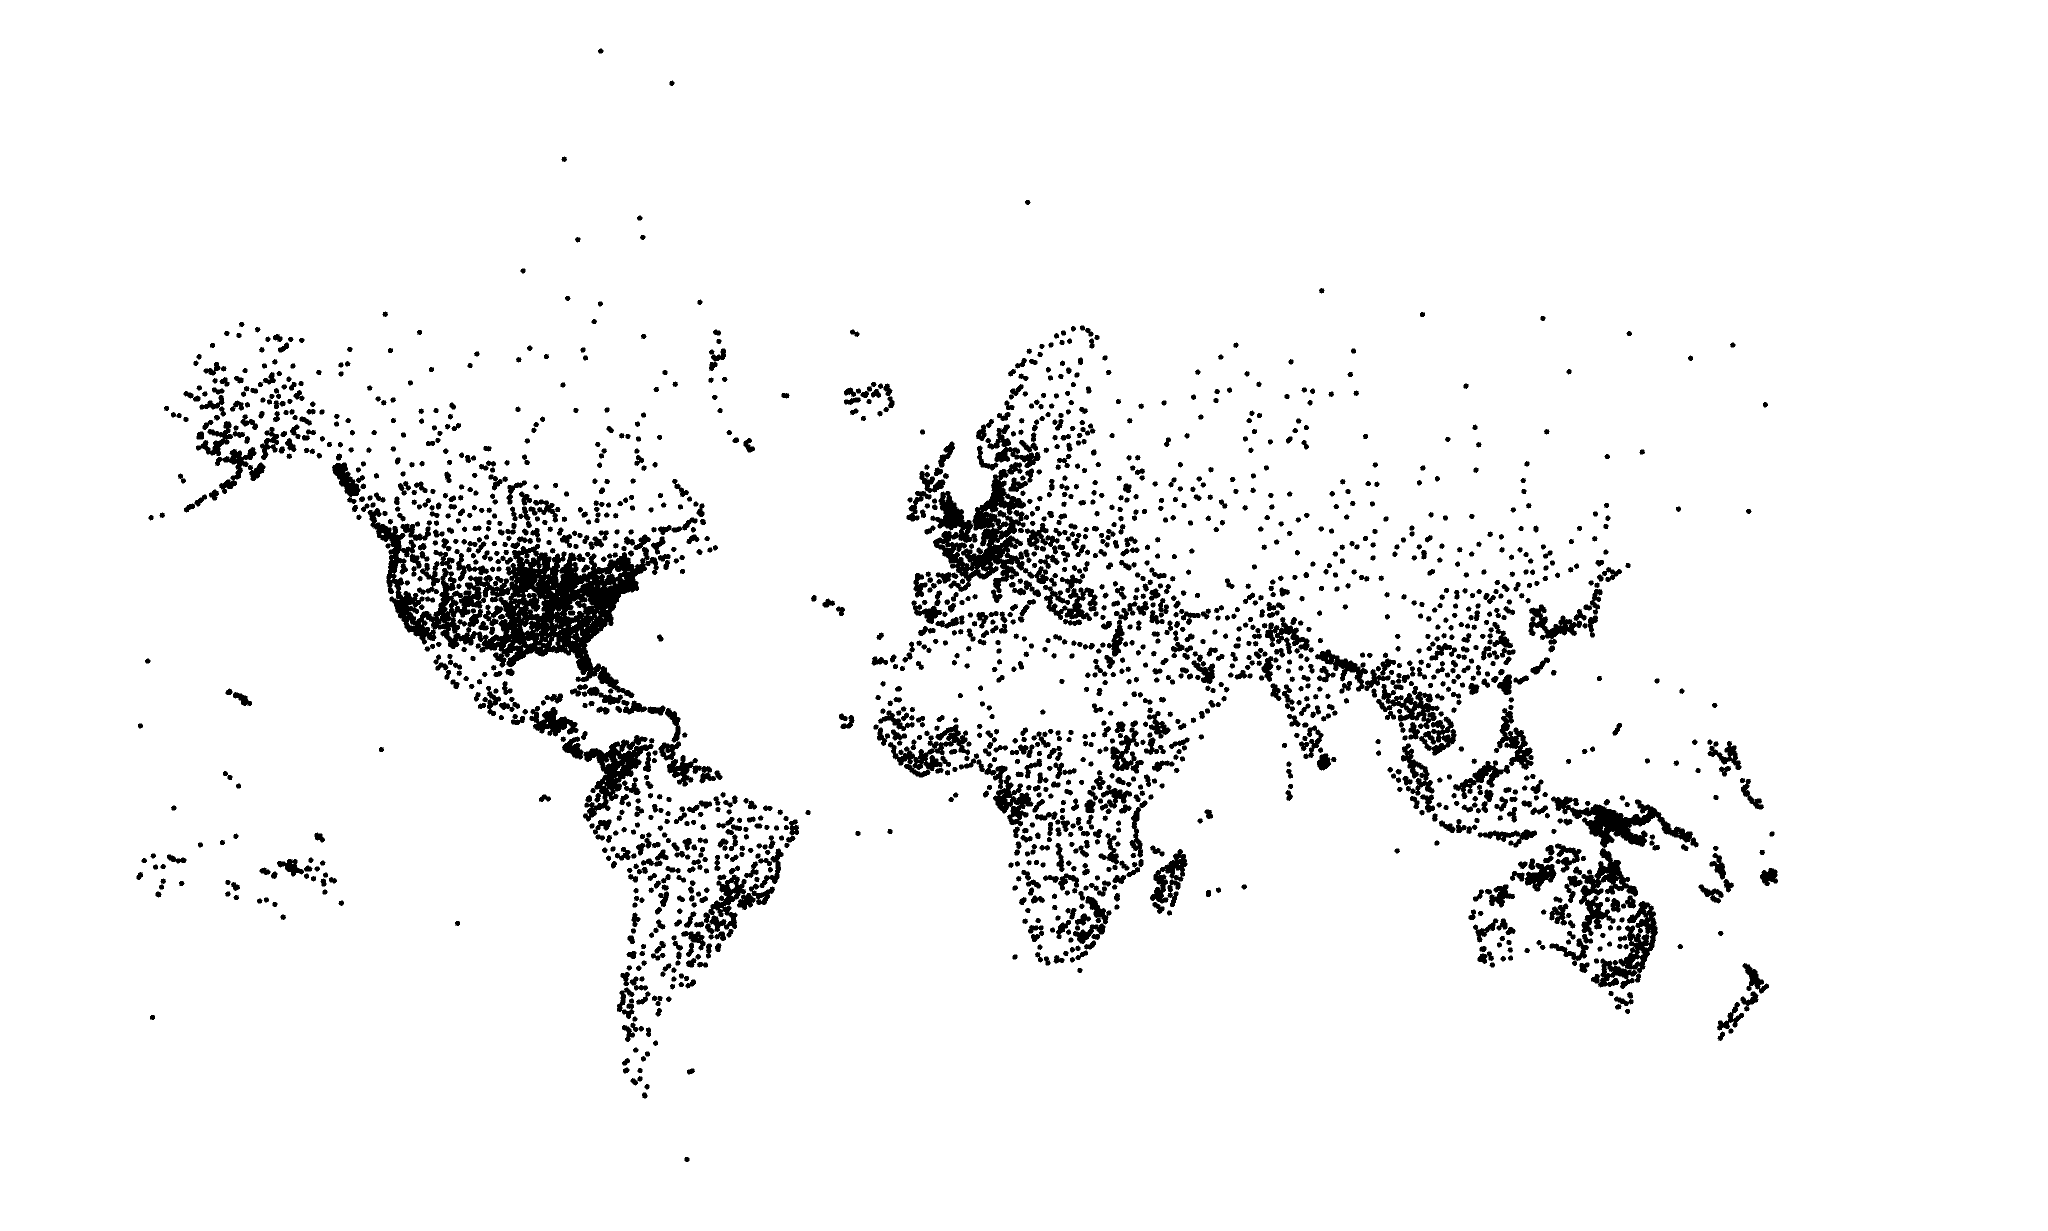
\includegraphics[width=\linewidth]{images/first-load-gephi.png}
    \caption{Erstes Laden der Flughäfen.}
    \label{fig:firstLoadGephi}
\end{figure}

Werden die Routen dazugeladen ergibt sich das Bild in Abb. \ref{fig:firstLoadGephiRoutes}

\begin{figure}
    \centering
    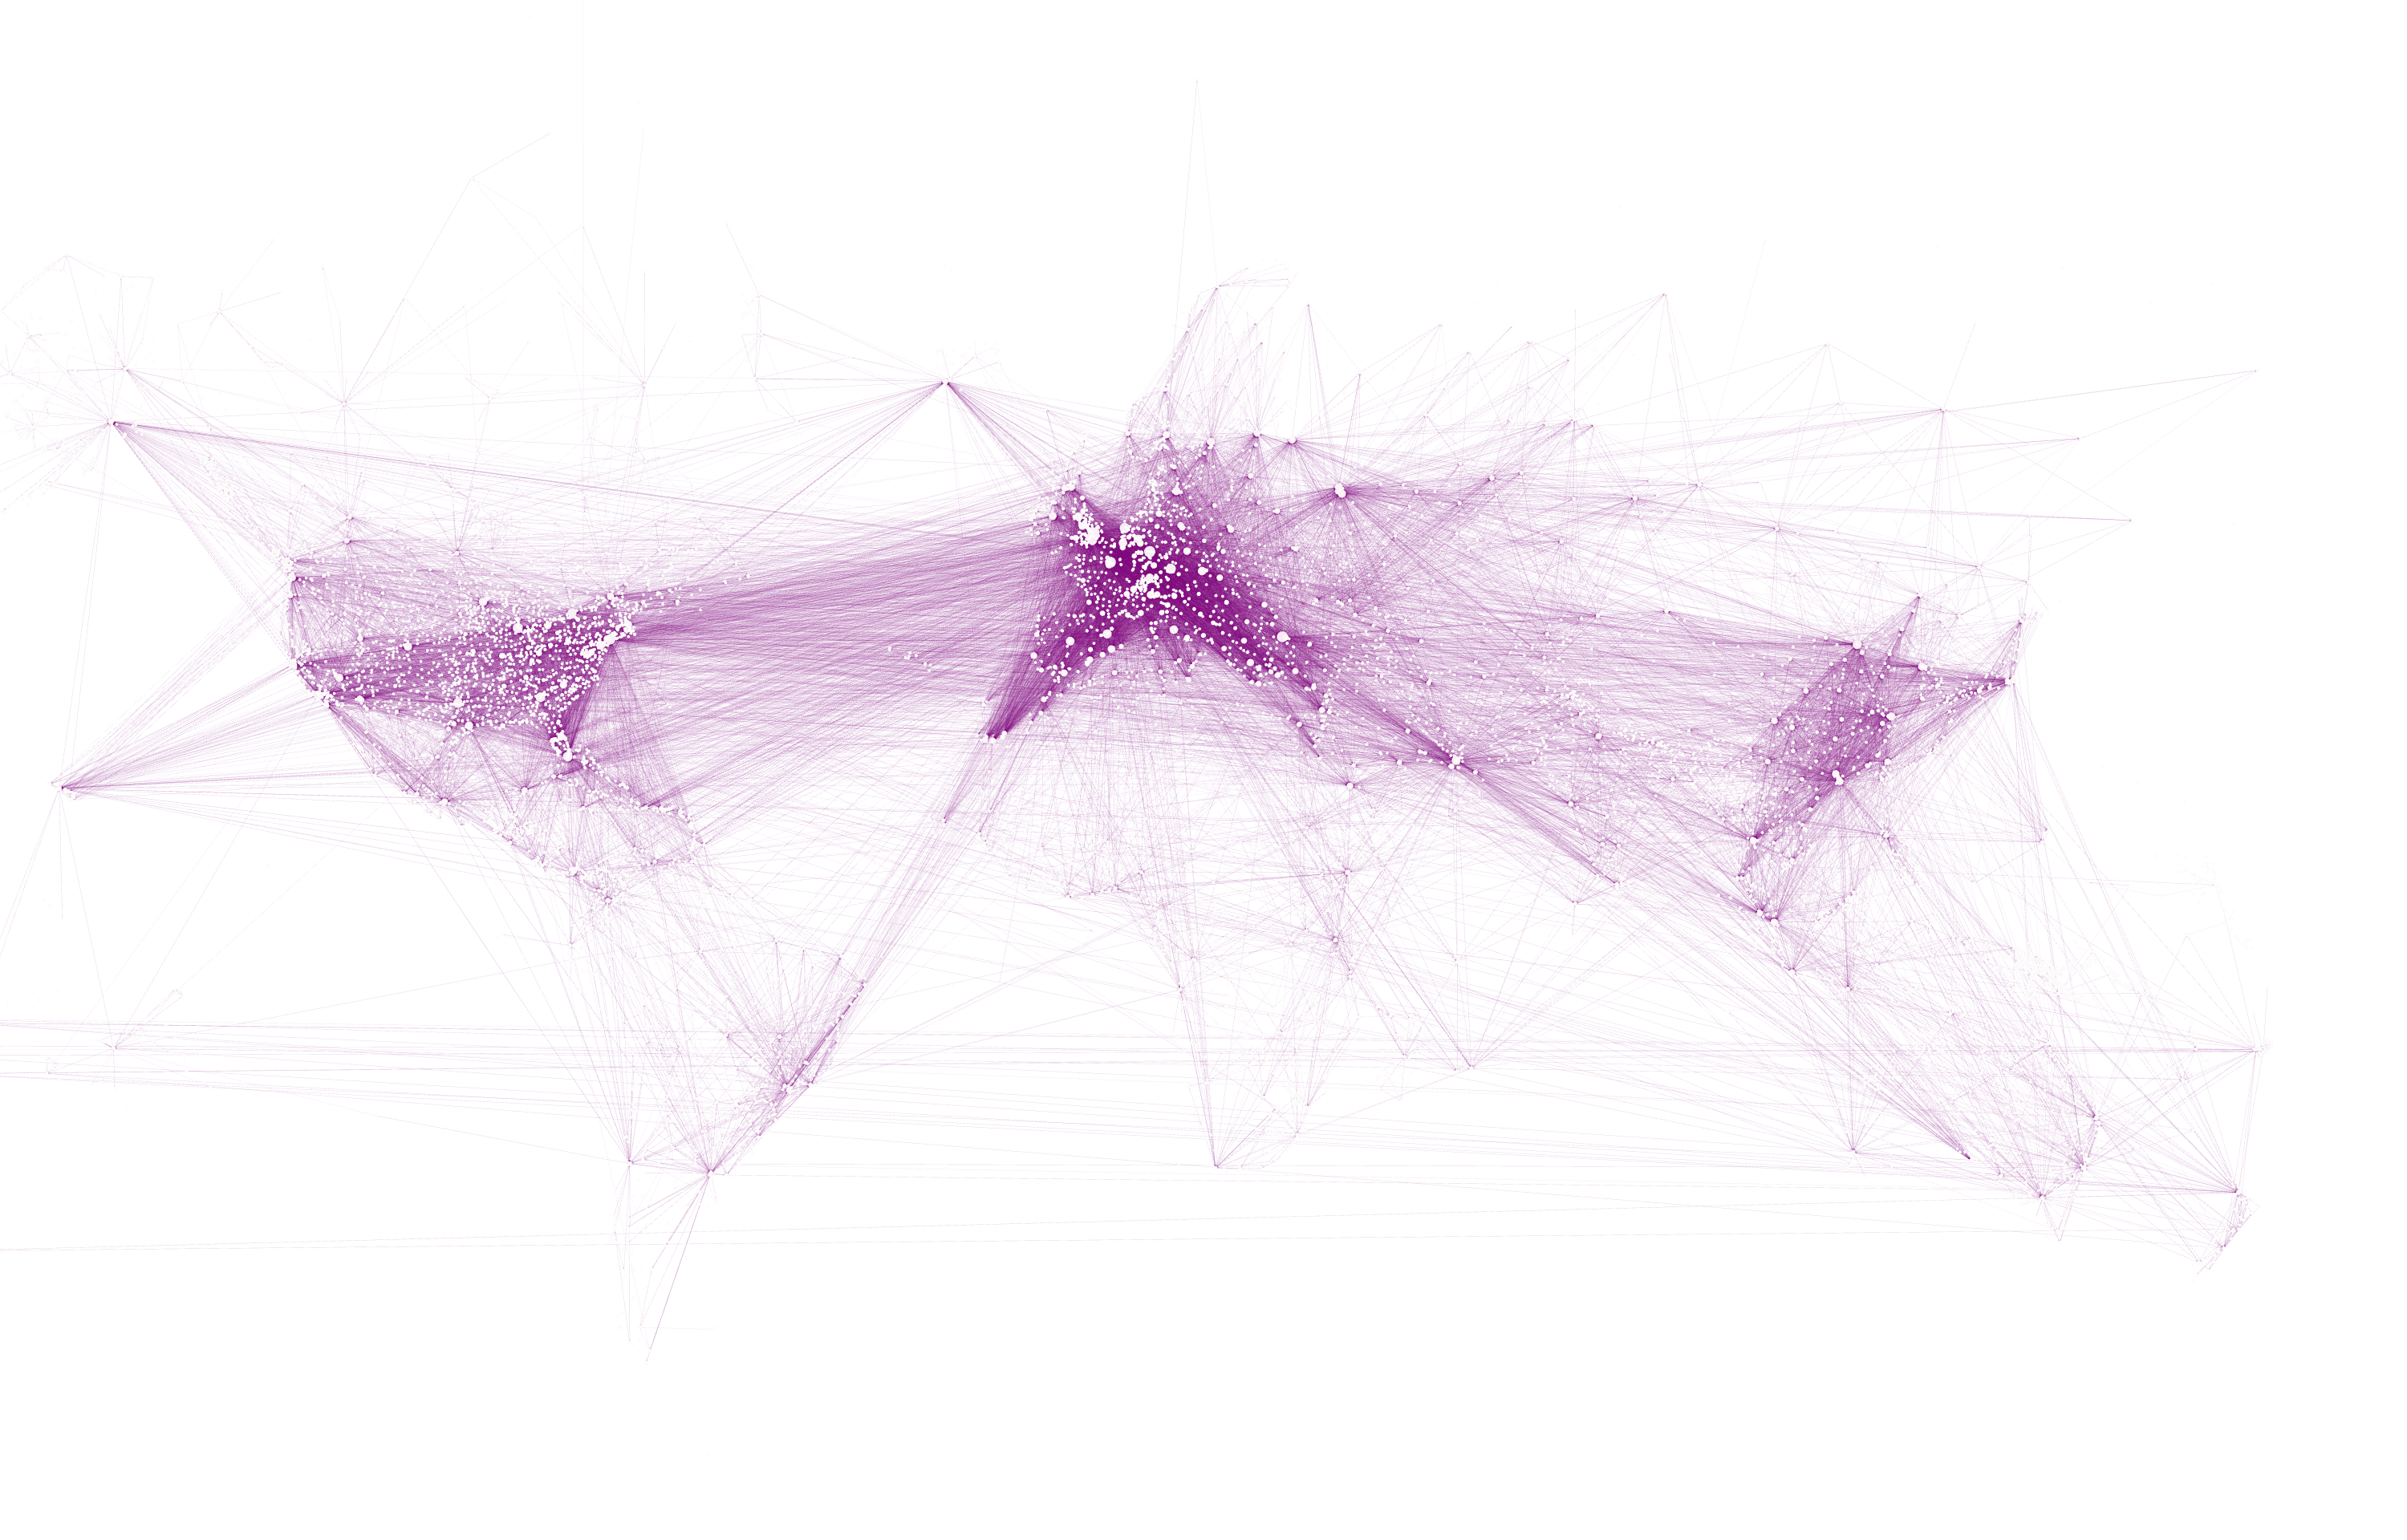
\includegraphics[width=\linewidth]{images/first-load-gephi-routes.png}
    \caption{Erstes Laden der Flughäfen.}
    \label{fig:firstLoadGephiRoutes}
\end{figure}

Bei der ersten Überprüfung fällt auf, dass sich unter den Flughäfen einige Bahnhöfe verstecken (siehe Abb. \ref{fig:railwayStations}).
Es ist nicht bekannt, weshalb diese Datensätze vorhanden sind.
Auch Aviation Edge schreibt nichts darüber.
Damit das Netzwerk möglichst nur Flughäfen und -felder enthält, werden die Bahnhöfe im Script entfernt.